\documentclass[11pt]{article}
\usepackage[utf8]{inputenc}
\usepackage[T1]{fontenc}
\usepackage{graphicx}
\usepackage{grffile}
\usepackage{longtable}
\usepackage{wrapfig}
\usepackage{rotating}
\usepackage[normalem]{ulem}
\usepackage{amsmath}
\usepackage{textcomp}
\usepackage{amssymb}
\usepackage{capt-of}
\usepackage{hyperref}
\usepackage{stmaryrd}
\usepackage{algorithm}
\usepackage{xcolor}
\usepackage{algorithmicx}
\usepackage[noend]{algpseudocode}
\author{Tom Gustafsson}
\date{\today}
 \hypersetup{
     colorlinks=true,
     linkcolor=purple,
     filecolor=purple,
     citecolor=purple,
     urlcolor=purple,
     }
\title{A technique for unstructured mesh generation via adaptive finite elements}
\begin{document}

\newcommand*\DNA{\textsc{dna}}

\newcommand*\Let[2]{\State #1 $\gets$ #2}
\algrenewcommand\algorithmicrequire{\textbf{Precondition:}}
\algrenewcommand\algorithmicensure{\textbf{Postcondition:}}

\maketitle

\begin{abstract}
  This article describes a concise algorithm for the generation of triangular
  meshes with the help of standard adaptive finite element methods.  We
  demonstrate that an adaptive finite element solver can produce quality meshes
  even for low quality initial meshes if a robust mesh smoothing algorithm is
  applied between the mesh refinement steps.  Thus, we propose that the adaptive
  process with smoothing can act as a general purpose triangular mesh generator.
  Finally, the mesh generator is applied to simulate an experimental creeping
  flow measurement analogous to electron current in graphene using the finite
  volume method.
\end{abstract}

\section{Introduction}
\label{sec:orge4667b0}

Many numerical methods for partial differential equations (PDE's), such as the
finite element method (FEM) and the finite volume method (FVM), are based on
splitting the domain of the solution into primitive shapes.  The collection of
the primitive shapes, i.e.~the computational mesh, is used to define the
discretization, e.g., in the FEM, the shape functions are polynomial in each
element of the mesh, and in the FVM, the discrete fluxes are defined over the
edges of the mesh.

This article describes a simple approach for the triangulation of
two-dimensional polygonal domains that are suitable for the discretization of
PDE's.  The process can be summarized as follows:
\begin{enumerate}
\item Find a constrained Delaunay triangulation (CDT) of the polygonal domain
      using the corner points as input vertices and the domain boundaries
      as constraints.
\item Solve the Laplace equation with the given triangulation
      and the FEM.
\item Split
      the triangles with the largest error indicator
      using adaptive mesh refinement techniques.
\item Apply mesh smoothing to the resulting triangulation.
\item Go to step 2.
\end{enumerate}
It is noteworthy that the steps 2, 3 and 5 correspond exactly to what is done in
any standard implementation of the adaptive FEM;
cf.~Verfürth~\cite{Verf_rth_2013} who calls it the \emph{adaptive process}.

The goal of this work is to demonstrate that if the mesh smoothing algorithm of
step 4 is chosen properly, the adaptive process tends to produce reasonable
meshes even if the initial mesh is of low quality.  Thus, we demonstrate that
the adaptive process---together with an implementation of the CDT and a robust
mesh smoothing algorithm---can act as a simple general purpose triangular mesh
generator.

\section{Prior work}
\label{sec:org7798f6d}

Two popular techniques for generating unstructured meshes are those based on the
\emph{advancing front technique}~\cite{L_hner_1988} or the \emph{Delaunay mesh
refinement}~\cite{Chew_1989, Ruppert_1995, Shewchuk_2002}.  In addition, there
exists several less known techniques such as \emph{quadtree
meshing}~\cite{Yerry_1983}, \emph{bubble packing}~\cite{Shimada_1995}, and
hybrid techniques combining some of the above~\cite{mavriplis1995advancing}.

Some existing techniques bear similarity to ours.  For example,
Bossen--Heckbert~\cite{bossen1996pliant} start also with a CDT and improve it by
relocating the nodes.  Instead of randomly picking nodes for relocation, we use
the finite element error indicator that guides the refinement.  Instead of doing
local modifications, we split simultaneously all triangles that have their error indicators
above a predefined threshold.

Persson--Strang~\cite{persson2004simple} describe another technique based on
iterative relocation of the nodes.  An initial mesh is given by a structured
background mesh which is then relaxed by intepreting the edges as a
precompressed truss structure.  The structure is forced inside a given
computational domain by expressing the boundary using signed distance functions
and using the signed distance as an external load.  In contrast to our approach,
the geometry description is implicit, i.e.~the boundary is defined as the zero
set of the signed distance function.

\section{Components of the mesh generator}
\label{sec:components}

The input to
our mesh generator is a sequence of \(N\) corner points
$$\mathcal{C} = (\mathcal{C}_1, \mathcal{C}_2, \dots, \mathcal{C}_N), \quad \mathcal{C}_j \in \mathbb{R}^2, \quad j = 1,\dots,N,$$
that form a polygon when connected by the edges
$$(\mathcal{C}_1, \mathcal{C}_2), (\mathcal{C}_2,\mathcal{C}_3),
\dots, (\mathcal{C}_{N-1}, \mathcal{C}_N), (\mathcal{C}_N,\mathcal{C}_1).$$
We do not allow self-intersecting polygons although
the algorithm can be generalized to polygons
with holes.
The corresponding polygonal domain is denoted
by \(\Omega_{\mathcal{C}} \subset \mathbb{R}^2\).

\subsection{Constrained Delaunay triangulation}
\label{sec:cdt}

A \emph{triangulation} of \(\Omega_{\mathcal{C}}\) is a collection of
nonoverlapping nondegenerate triangles whose union is exactly
\(\Omega_{\mathcal{C}}\).  Our initial triangulation \(\mathcal{T}_0\) is a
\emph{constrained Delaunay triangulation} (CDT) of the input vertices
\(\mathcal{C}\) with the edges \((\mathcal{C}_1, \mathcal{C}_2)\),
\((\mathcal{C}_2,\mathcal{C}_3)\), \(\dots\), \((\mathcal{C}_{N-1},
\mathcal{C}_N)\), \((\mathcal{C}_N, \mathcal{C}_1)\) constrained to be a part of
the resulting triangulation; cf.~Chew~\cite{Chew_1987} for the definition of a
CDT and a simple algorithm for its construction.

An example CDT of a polygon with a spiral-shaped boundary is given in
Figure~\ref{fig:cdt}. It is obvious that the CDT is not always a high quality
computational mesh due to the presence of arbitrarily small angles.  Thus, we
seek to improve the CDT by iteratively adding new triangles, and smoothing the
mesh.  Note that the remaining steps do not assume the use of CDT as the initial
triangulation---any conforming triangulation will suffice.

\begin{figure}[htbp]
  \centering
  \includegraphics[width=0.33\textwidth]{../image_19.png}
  \includegraphics[width=0.33\textwidth]{../image_5.png}
\caption{A spiral-shaped boundary approximated by linear segments and the corresponding
  CDT.  An example from the documentation of the
Triangle mesh generator~\cite{shewchuk1996triangle}.}
\label{fig:cdt}
\end{figure}

\subsection{Solving the Laplace equation}
\label{sec:poisson}

In order to decide on the placement of the new vertices and triangles, we solve
the Laplace equation\footnote{The choice of the Laplace equation is motivated by
the following heuristic observation: a \emph{quality mesh} is often synonymous with a \emph{good mesh for the
finite element solution of the Laplace equation}.} using the FEM and evalute the
corresponding a~posteriori error estimator.  The triangles matching
to the highest values of the error estimator are refined, i.e.~split
into smaller triangles.

The Laplace equation reads: find $u : \Omega_{\mathcal{C}} \rightarrow \mathbb{R}$ satisfying
\begin{alignat}{2}
-\Delta u &= 1 \quad && \text{in $\Omega_{\mathcal{C}}$,} \\
u &= 0 \quad && \text{on $\partial \Omega_{\mathcal{C}}$.}
\end{alignat}
The finite element method is used to numerically solve the
weak formulation: find \(u \in V\) such that
\begin{equation}
   \label{eq:weakform}
   \int_{\Omega_{\mathcal{C}}} \nabla u \cdot \nabla v \,\mathrm{d}x = \int_{\Omega_{\mathcal{C}}} v\,\mathrm{d}x \quad \forall v \in V,
\end{equation}
where
\(w \in V\) if \(w |_{\partial \Omega_{\mathcal{C}}} = 0\) and
$
   \int_{\Omega_{\mathcal{C}}} (\nabla w)^2 \,\mathrm{d}x < \infty.
$

We denote the \(k\)th triangulation of the
domain \(\Omega_{\mathcal{C}}\) by \(\mathcal{T}_k\), \(k=0,1,\dots\), and
use the piecewise linear polynomial space
$$V_h^k = \{ v \in V : v|_T \in P_1(T)~\forall T \in \mathcal{T}_k \},$$
where $P_1(T)$ denotes the set of linear polynomials over $T$.
The finite element method corresponding to the \(k\)th iteration reads:
find \(u_h^k \in V_h^k\) such that
\begin{equation}
   \label{eq:discweakform}
   \int_{\Omega_{\mathcal{C}}} \nabla u_h^k \cdot \nabla v_h \,\mathrm{d}x = \int_{\Omega_{\mathcal{C}}} v_h\,\mathrm{d}x \quad \forall v_h \in V_h^k.
\end{equation}
The local a posteriori error estimator
reads
\begin{equation}
        \eta_T(u_h^k) = \sqrt{h_T^2 |T|^2 + \frac12 h_T \int_{\partial T \setminus \partial \Omega_{\mathcal{C}}} (\llbracket \nabla u_h^k \cdot \boldsymbol{n} \rrbracket)^2 \,\mathrm{d}s}, \quad T \in \mathcal{T}_k,
\end{equation}
where $|T|$ is the area of the triangle $T$ and $h_T$ is the length of its longest edge, $\llbracket w \rrbracket |_{\partial T \setminus \partial \Omega_{\mathcal{C}}}$ denotes the jump in the values of
$w$ over $\partial T \setminus \partial \Omega_{\mathcal{C}}$, and $\boldsymbol{n}$ is a unit normal vector to
$\partial T$.
The error estimator $\eta_T$ is evaluated for each triangle
after solving \eqref{eq:discweakform}.
Finally, a triangle $T \in \mathcal{T}_k$ is marked for refinement if
\begin{equation}
  \label{eq:adaptivetheta}
   \eta_T > \theta \max_{T^\prime \in \mathcal{T}_k} \eta_{T^\prime},
\end{equation}
where $0 < \theta < 1$ is a parameter controlling the amount
of elements to split during each iteration.

\subsection{Red-green-blue refinement}
\label{sec:rgb}

The triangles marked for refinement by the rule \eqref{eq:adaptivetheta} are
split into four.  In order to keep the rest of the triangulation conformal,
i.e.~to not have any hanging nodes, the neighboring triangles are split into two or
three by the so-called red-green-blue (RGB)
refinement; cf.~Carstensen~\cite{carstensen2004adaptive}.
Application of the RGB refinement to the example of Figure~\ref{fig:cdt}
is depicted in Figure~\ref{fig:firstrgb}.

\begin{figure}[htbp]
\centering
\includegraphics[width=0.32\textwidth]{../image_5.png}
\includegraphics[width=0.32\textwidth]{../image_6.png}
\caption{(Left.) The initial triangulation. (Right.) The resulting mesh
after a solve of \eqref{eq:discweakform} and an adaptive RGB refinement.}
\label{fig:firstrgb}
\end{figure}

\subsection{Centroidal patch triangulation smoothing}
\label{sec:cpt}

We use a mesh smoothing approach introduced by Chen--Holst~\cite{Chen_2011} who
refer to the algorithm as \emph{centroidal patch triangulation} (CPT) smoothing.
The idea is to repeatedly move the interior vertices to the area-weighted
averages of the barycenters of the surrounding triangles.  The CPT smoothing is
combined with an edge flipping algorithm, also described in
Chen--Holst~\cite{Chen_2011}, to improve the quality of the resulting
triangulation.  The mesh smoother is applied to the spiral-shaped domain example 
in Figure~\ref{fig:firstsmooth}.

\begin{algorithm}[H]
  \caption{Mesh smoother}
  \begin{algorithmic}[1]
    \Require{$\mathcal{T}$ is a triangular mesh}
    \Require{$S$ is the total number of smoothing iterations}
    \Statex
    \Function{CPT}{$\mathcal{T}$}
    \Let{$\mathcal{T}_0$}{$\textsc{CDT}(\mathcal{C}$)}
    \For{$k \gets 1 \textrm{ to } M$}
    \Let{$\mathcal{T}_k^\prime$}{$\textsc{RGB}(\mathcal{T}_{k-1},\{\eta_T : T \in \mathcal{T}_{k-1}\})$}
    \Let{$\mathcal{T}_k$}{$\textsc{CPT}(\mathcal{T}_k^\prime)$}
    \EndFor
    \State \Return{$\mathcal{T}_N$}
    \EndFunction
  \end{algorithmic}
\end{algorithm}

\begin{figure}[htbp]
\centering
\includegraphics[width=0.32\textwidth]{../image_6.png}
\includegraphics[width=0.32\textwidth]{../image_7.png}
\caption{(Left.) Once adaptively refined triangulation. (Right.) The resulting
  triangulation after smoothing.}
\label{fig:firstsmooth}
\end{figure}

\section{The mesh generation algorithm}
\label{sec:orgff9b6c1}

In previous sections we gave an overview of all the components of the mesh
generation algorithm.  The resulting mesh generator is now summarized in
Algorithm~\ref{alg:meshgen}.  The total number of refinements $M$ is a constant
in order to guarantee the termination of the algorithm.  Nevertheless, in practice
the refinement loop should be terminated when a quality criterion is
satisfied, e.g., when the average minimum angle of the triangles
is above a predefined threshold.
The entire mesh generation process for the spiral-shaped domain
example is given in Figure~\ref{fig:spiralexample}.


\begin{figure}[htbp]
  \centering
  \includegraphics[width=0.24\textwidth]{../image_19.png}
  \includegraphics[width=0.24\textwidth]{../image_5.png}
  \includegraphics[width=0.24\textwidth]{../image_6.png}
  \includegraphics[width=0.24\textwidth]{../image_7.png}\\
  \includegraphics[width=0.24\textwidth]{../image_8.png}
  \includegraphics[width=0.24\textwidth]{../image_9.png}
  \includegraphics[width=0.24\textwidth]{../image_10.png}
  \includegraphics[width=0.24\textwidth]{../image_11.png}\\
  \includegraphics[width=0.24\textwidth]{../image_12.png}
  \includegraphics[width=0.24\textwidth]{../image_13.png}
  \includegraphics[width=0.24\textwidth]{../image_14.png}
  \includegraphics[width=0.24\textwidth]{../image_15.png}\\
  \includegraphics[width=0.24\textwidth]{../image_16.png}
  \includegraphics[width=0.24\textwidth]{../image_17.png}
  \caption{The entire mesh generation process for the spiral-shaped domain
    example from left-to-right, top-to-bottom.}
\label{fig:spiralexample}
\end{figure}


\begin{algorithm}[H]
  \caption{Triangular mesh generator}
  \label{alg:meshgen}
  \begin{algorithmic}[1]
    \Require{$\mathcal{C}$ is a sequence of domain corner points}
    \Require{$M$ is the total number of refinements}
    \Statex
    \Function{Generate}{$\mathcal{C}$}
    \Let{$\mathcal{T}_0$}{$\textsc{CDT}(\mathcal{C}$)}
    \For{$k \gets 1 \textrm{ to } M$}
    \Let{$\mathcal{T}_k^\prime$}{$\textsc{RGB}(\mathcal{T}_{k-1},\{\eta_T : T \in \mathcal{T}_{k-1}\})$}
    \Let{$\mathcal{T}_k$}{$\textsc{CPT}(\mathcal{T}_k^\prime)$}
    \EndFor
    \State \Return{$\mathcal{T}_N$}
    \EndFunction
  \end{algorithmic}
\end{algorithm}


\section{Implementation and examples}

We implemented the mesh generator in Python for computational experiments.  Our
implementation is referred to as \verb|adaptmesh| and is archived in Zenodo~??.
The implementation relies heavily on the scientific Python
ecosystem~\cite{virtanen2020scipy}.  It includes source code from \verb|tri|
\cite{tri} (CDT) and the early MIT licensed versions of \verb|optimesh|
\cite{optimesh} (CPT smoothing) and \verb|meshplex| \cite{meshplex} (edge
flipping).  Moreover, it dynamically imports modules from \verb|scikit-fem|
\cite{gustafsson2020scikit} (RGB refinement) and \verb|matplotlib|
\cite{hunter2007matplotlib} (visualization).  Some examples are given in
Figure~\ref{fig:moreexamples}.  Note that by default \verb|adaptmesh| uses the
average triangle quality as a stopping criterion which can lead to individual
low quality triangles.  Using the minimum triangle quality will lead to more
refined meshes.

\begin{figure}[htbp]
  \centering
  \includegraphics[width=0.32\textwidth]{../image_1.png}
  \includegraphics[width=0.32\textwidth]{../image_2.png}
  \includegraphics[width=0.32\textwidth]{../image_4.png}\\
  \includegraphics[width=0.22\textwidth]{../image_21.png}
  \includegraphics[width=0.32\textwidth]{../image_22.png}
  \includegraphics[width=0.32\textwidth]{../image_23.png}
  \caption{Some example meshes generated using \texttt{adaptmesh}.}
\label{fig:moreexamples}
\end{figure}

\section{An example application}

As an example application, we simulate the experiment of a
microfluidic device from
Mayzel--Steinberg--Varshney~\cite{mayzel2019stokes}
which is analogous to electron transport in two-dimensional
conductive materials such as graphene.
The governing equation is the Stokes system
\begin{equation}
  \left\{
  \begin{aligned}
    -\nabla \cdot (2\mu\,\varepsilon(\nabla u)) + \nabla p &= 0, \\
    \nabla \cdot u &= 0,
  \end{aligned}
  \right.
\end{equation}
where the unknowns are the velocity $u : \Omega \rightarrow \mathbb{R}^2$ and
the pressure $p : \Omega \rightarrow \mathbb{R}$, the viscosity $\mu > 0$ is
given, and $\varepsilon(\nabla u) = \tfrac12(\nabla u + \nabla u^T)$ is the
rate-of-strain tensor.

The boundary $\partial \Omega$ of the computational domain $\Omega \subset
\mathbb{R}^2$ is extracted from a photograph of the experiment and given as an
input to the mesh generator; the photograph is given in the top-left panel and
the resulting computational mesh in the top-right panel of
Figure~\ref{fig:esimerkki}.  In order to simplify the problem we choose the
computational domain so that the left boundary corresponds approximately to the
vertical streamlines in the micro-particle image velocimetry (bottom-left
panel), i.e.~the computational domain is enclosed in the red rectangle.  This
allows using the Dirichlet boundary condition $u_x = 0$, $u_y = -U$, $U > 0$, on
the left boundary.

\begin{figure}[htbp]
\centering
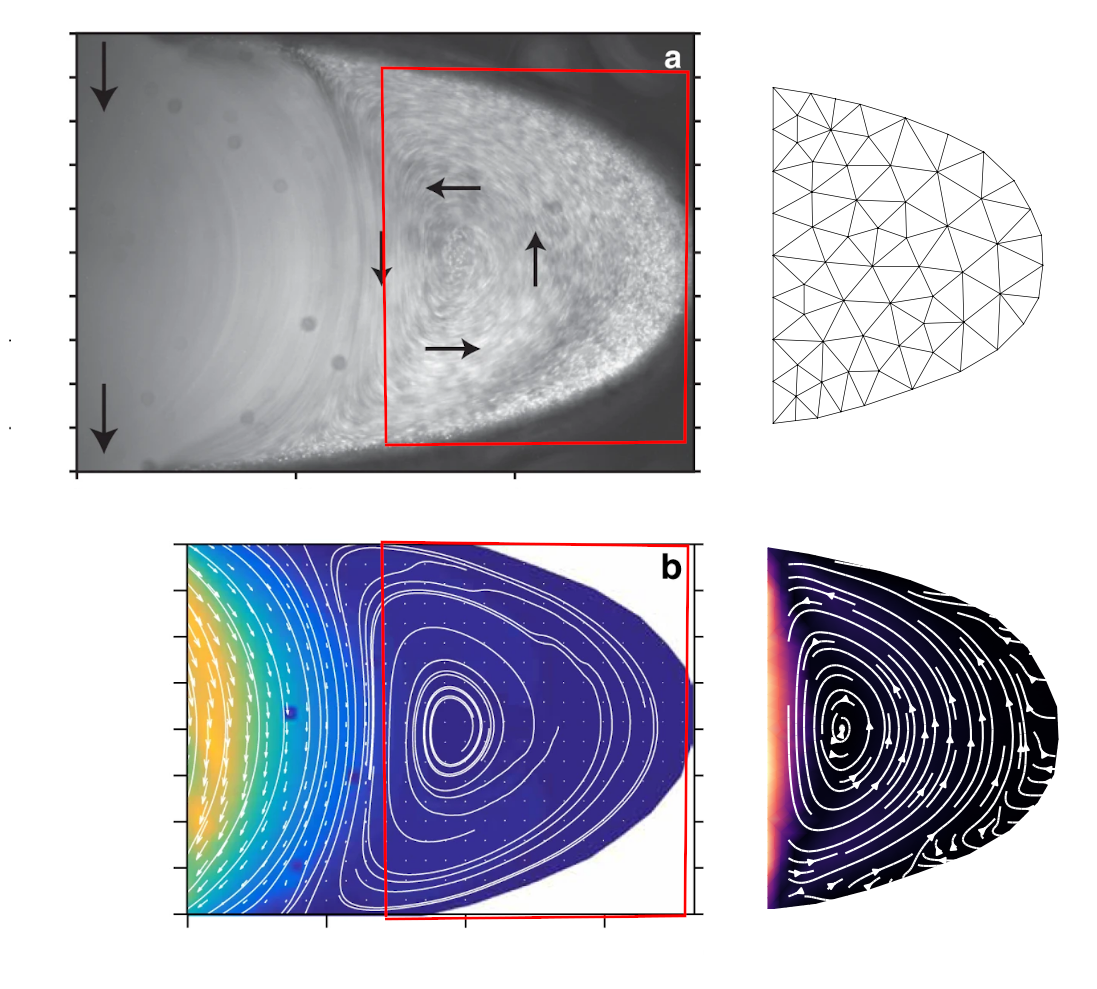
\includegraphics[width=\textwidth]{./esimerkki_vertailu.png}
\caption{(Top-left.) A photograph of the experiment with the particles trapped
  inside a microfluidic device;
  cf.~Mayzel--Steinberg--Varshney~\cite{mayzel2019stokes} for more details.
  (Top-right.) The mesh resulting from our mesh generator. (Bottom-left.)  The
  experimental streamlines obtained from micro-particle image velocimetry.
  (Bottom-right.) The computational streamlines calculated using
  FiPy~\cite{FiPy2009}.  The images on the left panel are cropped from the
  figures in Mayzel--Steinberg--Varshney~\cite{mayzel2019stokes} with the red
  rectangles added later by the author of this paper.  These images (the
  original and the modified ones) are licensed under Creative Commons
  Attribution 4.0 International License
  (see~\url{https://creativecommons.org/licenses/by/4.0/}).}
\label{fig:esimerkki}
\end{figure}

\section{Conclusions and future work}
\label{sec:org615e973}

\bibliographystyle{unsrt}
\bibliography{mesh}

\end{document}
